\documentclass[a4paper, 12pt]{article}%тип документа

%отступы
\usepackage[left=1.5cm,right=1cm,top=2cm,bottom=3cm,bindingoffset=0cm]{geometry}
\setlength{\parindent}{5ex}

%Русский язык
\usepackage[T2A]{fontenc} %кодировка
\usepackage[utf8]{inputenc} %кодировка исходного кода
\usepackage[english,russian]{babel} %локализация и переносы

%Вставка картинок
\usepackage{graphicx}
\graphicspath{{pictures/}}
\DeclareGraphicsExtensions{.pdf,.png,.jpg,.jfif}
\usepackage{wrapfig}

%Графики
\usepackage{pgfplots}
\pgfplotsset{compat=1.9}

%Математика
\usepackage{amsmath, amsfonts, amssymb, amsthm, mathtools}

%Таблицы
\usepackage{longtable} 
\usepackage{float}

%Римские цифры
\newcommand{\RomanNumeralCaps}[1]{\uppercase\expandafter{\romannumeral#1}}

\usepackage{multirow}


\begin{document}
	\begin{titlepage}
		\begin{center}
			\textsc{Федеральное государственное автономное образовательное учреждение высшего образования«Московский физико-технический институт (национальный исследовательский университет)»\\[5mm]
			}
			
			\vfill
			
			\textbf{Отчёт по лабораторной работе 5.1.3\\[3mm]
				Излучение рассеяния медленных электронов на атомах (Эффект Рамзауэра)
				\\[50mm]
			}
			
		\end{center}
		
		\hfill
		\begin{minipage}{.5\textwidth}
			Выполнил студент:\\[2mm]
			Сериков Василий Романович\\[2mm]
			группа: Б03-102\\[5mm]
			
		\end{minipage}
		\vfill
		\begin{center}
			Москва, 2023 г.
		\end{center}
		
	\end{titlepage}
	
	\newpage
	\setcounter{page}{2}
	\textbf{Аннотация}\\
	
	\textbf{Цель работы: }\\
	
	Исследовать энергетические зависимости вероятности рассеяния электронов атомами ксенона, определить энергии электронов, при которых наблюдается просветление ксенона и оценить размер его внешней электронной оболочки. \\
	
	\textbf{Теория: }\\
	
	Распределение вероятности обнаружить частицу в какой-то области пространства $d V$ описывается в квантовой физике комплексной волновой функцией $\psi(\vec{r}): d w=|\psi|^2 d V$. Волновая функция стационарного состояния (состояния с определённой энергией $E$ ) подчиняется уравнению Шредингера $\quad-\frac{\hbar^2}{2 m} \Delta \psi+U(\vec{r}) \psi=E \psi$, где $U(\vec{r}) \quad-$ потенциальная энергия частицы.
	
	От волновой функции требуются:
	1. непрерывность, так как скачок волновой функции будет соответствовать резкому нефизическому скачку в распределении вероятности
	2. гладкость (за исключением нефизического, но полезного случая бесконечно высокой стенки), так как скачок производной соответсвует нефизическому скачку среднего импульса $\langle\vec{p}\rangle=-i \hbar \int \psi^* \vec{\nabla} \psi d V \quad$ на границе
	
	Нормировка волновой функции $\int \psi^* \psi d V=1$, выражающая математическое требование суммы всех вероятностей, равной 1 , применяется при финитном движении частицы (волновая функция отлична от нуля в ограниченной области пространства).
	
	Для свободной частицы ( $U=0)$ уравнение Шредингера имеет решение вида плоской волны $\psi=C e^{i \vec{r} \vec{r}}$. Для нормировки такого решения удобно выразить поток частиц (число частиц, пересекающих площадку $d S$ за время $d t$ :
	$$
	j=\frac{d N}{d S d t}=\frac{|\psi|^2 d V}{d S d t}=\frac{|\psi|^2 d S \frac{p}{m} d t}{d S d t}=\frac{\hbar k}{m}|\psi|^2
	$$
	
	Рассмотрим одномерную задачу с потенциалом
	$$
	U(x)=\left\{\begin{array}{c}
		0, x<0 \\
		-U_0 0<x<l \\
		0, x>l
	\end{array} .\right.
	$$
	
	Такой потенциал называют потенциальной ямой глубиной $U_0$ и шириной $l$.
	Пусть на такую яму из минус бесконечности падает поток частиц. Определим долю частиц, прошедших через яму.
	
	Одномерное уравнение Шредингера $-\frac{\hbar^2}{2 m} \psi^{\prime \prime}+(U-E) \psi=0$ в областях $\quad x<0 \quad$ и $\quad x>l$ (где $U=0$ ) имеет решение вида $\psi=A e^{i k_1 x}+B e^{-i k_1 x}$, где $k_1^2=\frac{2 m E}{\hbar^2}$. В области $0<x<l \quad\left(\right.$ где $\left.U=-U_0\right) \quad \psi=A e^{i k_2 x}+B e^{-i k_2 x}$, где $k_2^2=\frac{2 m\left(E+U_0\right)}{\hbar^2}$
	
	Слагаемые с положительным знаком в экспоненте соответствуют волне, распространяющейся слева направо. Слагаемые с отрицательным знаком - волне, распространяющейся справа налево.
	
	В силу произвольности выбора падающего потока частиц, можно положить одну из констант равной произвольному числу. Удобно таким образом отнормировать падающий поток. Кроме того, после ямы имеет физический смысл только решение, распространяющееся слева направо (не от чего отражаться обратной волне).
	
	Таким образом, решения для волновой функции надо искать в виде:
	$$
	\psi=\left\{\begin{array}{c}
		e^{i k_1 x}+A e^{-i k_1 x}, x<0 \\
		C_1 e^{i k_1 x}+C_2 e^{-i k_1 x}, 0<x<l . \\
		B e^{i k_1 x}, x>l
	\end{array} .\right.
	$$
	
	Требования непрерывности и гладкости при $x=0$ и $x=l \quad$ приводят к системе линейных уравнений:
	$$
	\begin{gathered}
		1+A=C_1+C_2 \\
		C_1 e^{i k_2 l}+C_2 e^{-i k_2 l}=B e^{i k_1 l} \\
		k_1(1-A)=k_2\left(C_1-C_2\right) \\
		k_2\left(C_1 e^{i k_2 l}-C_2 e^{-i k_2 l}\right)=k_1 B e^{i k_1 l}
	\end{gathered}
	$$
	
	Система позволяет найти все коэффициенты, но для нахождения коэффициента прохождения (или коэффициента отражения) достаточно найти амплитуду прошедшей (отражённой) волны $B$ ( $A)$. После прямолинейных преобразований получаем:
	$$
	B=\frac{4 k_1 k_2 e^{-i k_1 l}}{\left(k_1+k_2\right)^2 e^{-i k_2 l}-\left(k_1-k_2\right)^2 e^{i k_1 l}}
	$$
	
	Коэффициент прохождения над ямой определяется отношением потоков падающих и прошедших частиц, то есть ${ }^1$ :
	$$
	D=|B|^2=B B^*=\frac{16 k_1^2 k_2^2}{\left(k_1+k_2\right)^4+\left(k_1-k_2\right)^4-\left(k_1+k_2\right)^2\left(k_1-k_2\right)^2\left(e^{2 i k_2 l}+e^{-2 i k_2 l}\right)} .
	$$
	
	\textbf{Экспериментальная установка: }\\
	
	В работе используется тиратрон ТГЗ-01/1.3Б, заполненный инертным газом. Электроны, эмитируемые катодом, ускоряются напряжением V, затем рассеиваются на атомах инертного газа. Эти электроны попадают на сетку, а оставшиеся попадают на анод и создают анодный ток.
	
	Уравнение ВАХ 
	\begin{equation}\label{3}
		I_\text{a} = I_0 \exp\left( - C w(V) \right),
	\end{equation}

	\begin{figure}[H]
		\centering
		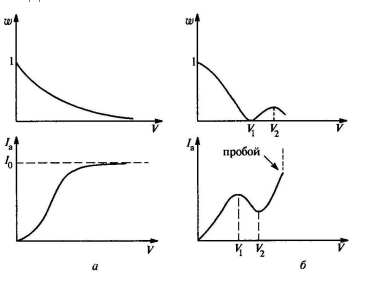
\includegraphics[width=0.6\linewidth]{compare}
		\caption{Вероятность рассеяния электрона и ВАХ тератрона при классическом рассмотрении (а) и квантовом (б)}
	\end{figure}
	где $I_0 = eN_0$ -- ток катода, $I_\text{a} = eN_a$ -- ток анода, $C = Ln_\text{a} \Delta_\text{a}$($L$ --  расстояние между катодом и анодом, $\Delta_\text{a}$ -- площадь поперечного сечения атома, $n_\text{a}$ -- концентрация газа в лампе), $w(V)$ -- вероятность рассеяния на атоме.
	Зависимость вероятности рассеяния электрона от его энергии
	\[\tag{5a}\label{5a}
	w(V) = -\dfrac{1}{C}\ln \dfrac{I_\text{a}(V)}{I_0}.
	\]
	
	\begin{figure}[H]
		\centering
		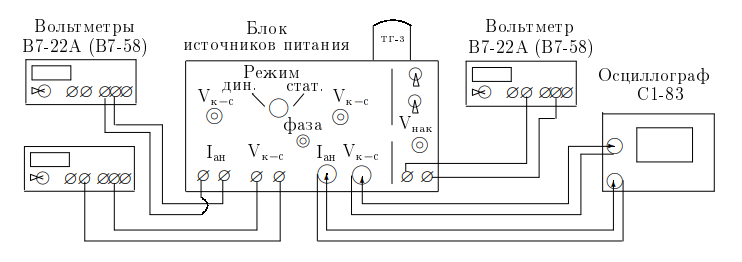
\includegraphics[width=1\linewidth]{ust1}
		\caption{Блок-схема установки}
	\end{figure}

	\begin{figure}[H]
		\centering
		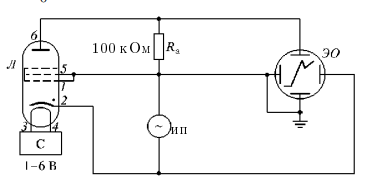
\includegraphics[width=0.6\linewidth]{ust}
		\caption{Принципиальная схема установки}
	\end{figure}
	
	
	\newpage
	
	\textbf{Ход работы: }\\
	
	\begin{enumerate}
	
	\item Получим изображение ВАХ на экране осциллографа в динамическом режиме. Полученная  картинка для двух различных значений напряжения накала лампы изображены на Рис4. и Рис5.
	
	\begin{figure}[H]
		\centering
		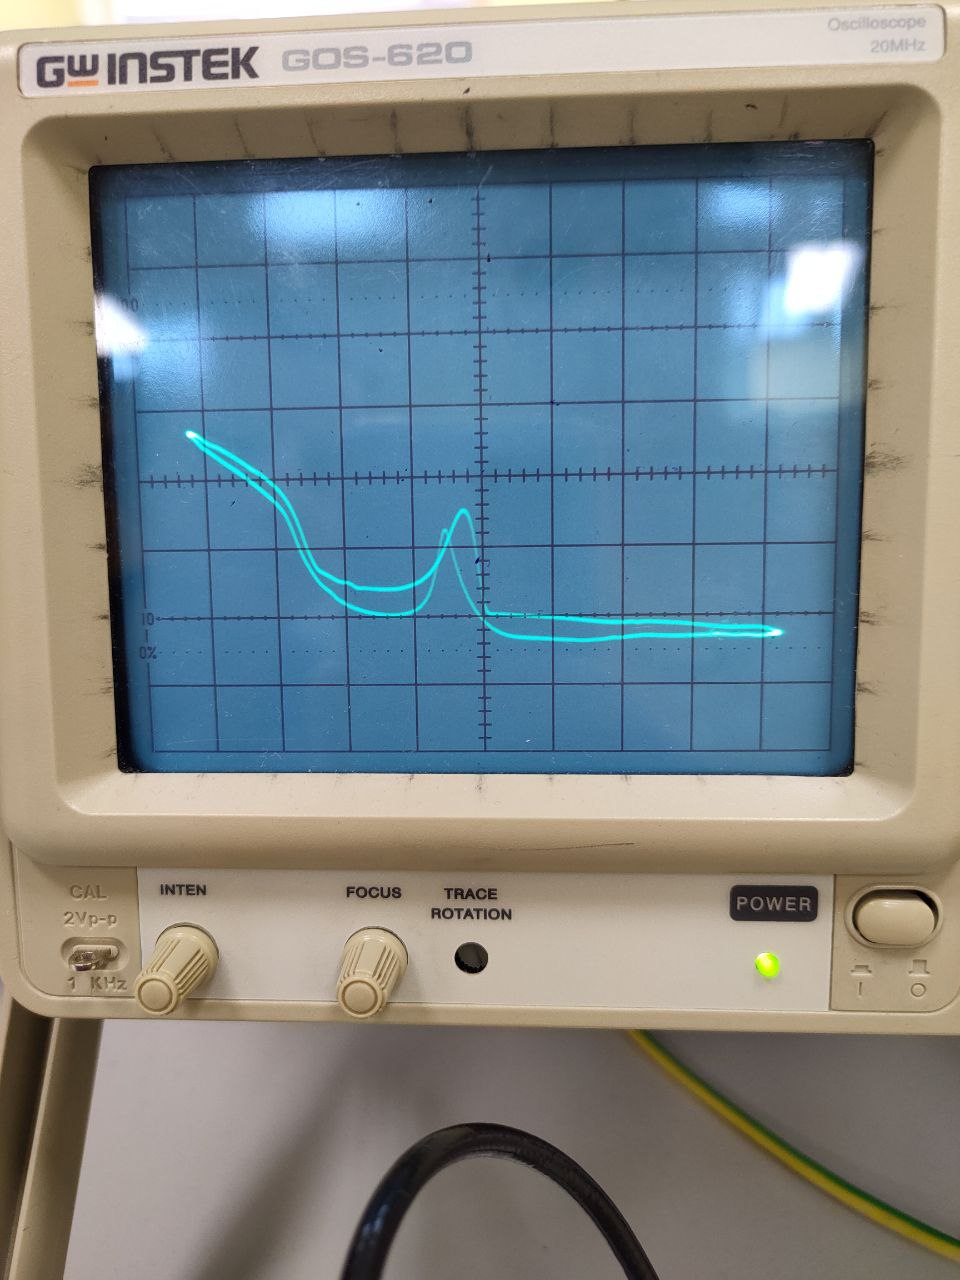
\includegraphics[width=0.6\linewidth]{2.519.jpeg}
		\caption{Осциллограмма при напряжении накала $V = 2,52 \pm0,01$ В.  Цена деления по оси абсцисс 5 В/дел.}
	\end{figure}

	\begin{figure}[H]
		\centering
		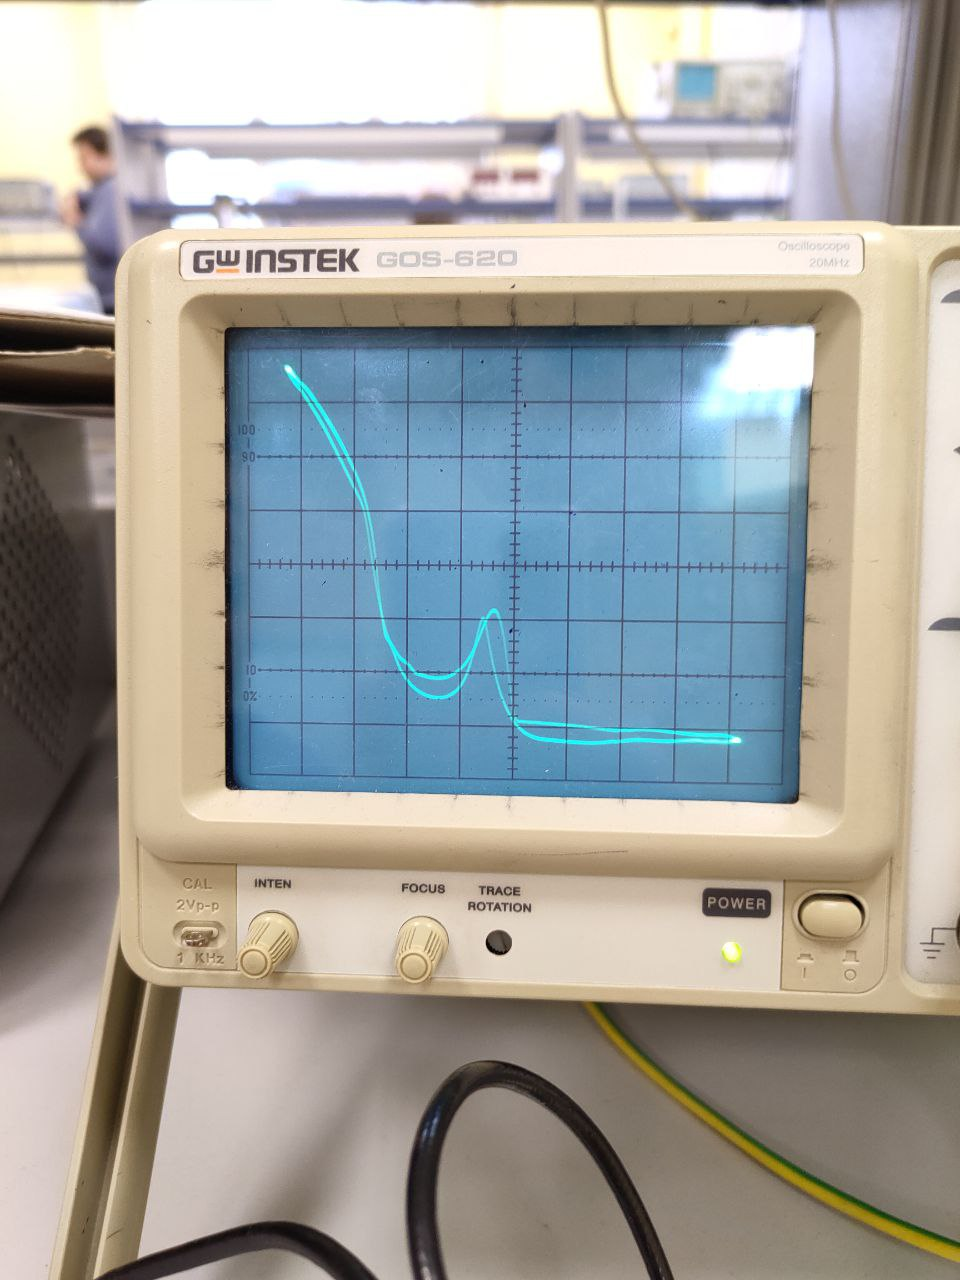
\includegraphics[width=0.6\linewidth]{2.794.jpeg}
		\caption{Осциллограмма при напряжении накала $V = 2,79 \pm0,01$ В. Цена деления по оси абсцисс 5 В/дел.}
	\end{figure}

	
	\item По полученным осциллограммам определим напряжение между катодом и сеткой, соответствующее первому максимуму и минимуму (отсчет максимумов и минимумов начинается справа налево).
	
	Оценим напряжение пробоя, соответствующее резкому скачку тока в конце кривой.
	
	Полученные значения занесем в таблицу 1.
	
	\begin{longtable}{|c|c|c|c|c|c|c|}
		\hline
		& $\Delta_{max}$, дел. & $\Delta_{min}$, дел. & $\Delta_{\text{проб.}}$, дел. & $\Delta_{max}$, В & $\Delta_{min}$, В & $\Delta_{\text{проб.}}$, В \\ \hline
		$V_1 = 2,79$ В & 0,5 & 1,3 & 2,4 & 2,5 & 6.5 & 12 \\ \hline 	
		$V_1 = 2,52$ В & 0,5 & 1,2 & 2,4 & 2,5 & 6 & 12 \\ \hline
		
		\caption{Значения напряжений при первом максимуме и минимуме анодного тока и напряжение пробоя. Цена деления по оси абсцисс 5 В/дел. $\sigma_{\Delta} = 0,1$ дел. = 0,5 В}
	\end{longtable}
	
	\newpage
	\item По результатам измерений рассчитаем размер электронной оболочки атома инертного газа, заполняющего лампу, приняв $U_0$ = 2,5В.
	
	$$ l_1 = \frac{3}{4} \frac{h}{\sqrt{2m(E_2 + U_0)}} $$
	
	$$ l_2 = \frac{1}{2} \frac{h}{\sqrt{2m(E_1 + U_0)}} $$
	
	Также рассчитаем размер оболочки атома этого газа по формуле:
	
	$$ l_3 = \frac{h\sqrt{5}}{\sqrt{32m(E_2 - E_1)}} $$
	
	$$ \sigma_{l_1} = l_1\frac{3}{2} \cdot \frac{m}{2m(E_2 + U_0)} \sigma_{E_2} $$
	$$ \sigma_{l_2} = l_2 \frac{2m}{2m(E_1 + U_0)} \sigma_{E_1}$$
	$$ \sigma_{l_3} = l_3 \sqrt{ \left( \frac{1}{E_2 - E_1} \sigma_{E_1} \right)^2 + \left(  \frac{1}{E_2 - E_1} \sigma_{E_2} \right) ^2}$$
	
	\item Оценим глубину потенциальной ямы по формуле: 
	
	$$ U_0 = \frac{4}{5} E_2 - \frac{9}{5} E_1$$
	
	Результаты измерений пунктов 3-4 занесем в таблицу 2.
	
	\begin{longtable}{|c|c|c|c|c|}
		\hline
		$l_1$, \AA & $l_2$, \AA & $l_3$, \AA & $U_0$, эВ & $l_{\text{табл.}}$, \AA\\ \hline
		2,7 $\pm0,2$ & 3,1$\pm0,2$ & 3,4$\pm0,3$ & 0,7 $\pm0,5$ & 1\\ \hline
		\caption{Полученные значения для размера электронной оболочки атома ксенона в динамическом режиме}
	\end{longtable}
	
	\item Проведем измерения ВАХ тиратрона в статическом режиме для двух значений напряжения накала (тех же, что в динамическом режиме).
	Полученные результаты занесем в таблицу 3. Построим график $ I_a = f(V_c) $
	
	\begin{longtable}{|c|c|c|c|c|c|c|c|}
		\hline
		\multicolumn{4}{|c|}{$V_1$ = 2,770 В} & \multicolumn{4}{c|}{$V_2$ = 2,516 В} \\ \hline
		$V_\text{анод.}$, мВ & $V_\text{кат.-сет.}$, В &  $V_\text{анод.}$, мВ & $V_\text{кат.-сет.}$, В  & $V_\text{анод.}$, мВ & $V_\text{кат.-сет.}$, В  &  $V_\text{анод.}$, мВ & $V_\text{кат.-сет.}$, В  \\ \hline
		
		1,18  & 0,582 & 74,5  & 4,875 & 0,10   & 0,125 & 42,13 & 4,419 \\ \hline
		19,70 & 0,853 & 72,58 & 5,090 & 0,43   & 0,600 & 39,78 & 4,660 \\ \hline
		76,50 & 1,086 & 71,12 & 5,266 & 2,44   & 0,750 & 38,02 & 4,844 \\ \hline
		115,8 & 1,212 & 70,27 & 5,420 & 8,06   & 0,858 & 36,07 & 5,067 \\ \hline
		175,1 & 1,467 & 68,95 & 5,664 & 22,97  & 0,970 & 35,05 & 5,267 \\ \hline
		194,5 & 1,667 & 67,5  & 5,872 & 43,89  & 1,069 & 33,95 & 5,503 \\ \hline
		195,5 & 1,779 & 66.62 & 6,063 & 70,39  & 1,168 & 33,44 & 5,623 \\ \hline
		191,5 & 1,890 & 66,17 & 6,268 & 81,7   & 1,205 & 32,63 & 5,880 \\ \hline
		187,3 & 1,965 & 66,32 & 6,640 & 112,8  & 1,317 & 33,32 & 6,003 \\ \hline
		181,0 & 2,054 & 65,86 & 6,875 & 132,1  & 1,388 & 31,75 & 6,248 \\ \hline
		175,0 & 2,120 & 65,88 & 7,075 & 144,1  & 1,439 & 31,35 & 6,465 \\ \hline
		165,2 & 2,250 & 65,81 & 7,248 & 164,2  & 1,545 & 31,29 & 6,672 \\ \hline
		153,7 & 2,403 & 66,50 & 7,491 & 173,6  & 1,620 & 31,05 & 6,861 \\ \hline
		145,7 & 2,515 & 67,36 & 7,650 & 180,80 & 1,721 & 30,90 & 7,061 \\ \hline
		135,2 & 2,680 & 68,50 & 7,832 & 180,80 & 1,820 & 30,91 & 7,213 \\ \hline
		129,8 & 2,774 & 70,38 & 8,024 & 182,19 & 1,925 & 31,07 & 7,478 \\ \hline
		124,4 & 2,876 & 73,48 & 8,263 & 172,22 & 2,014 & 31,35 & 7,652 \\ \hline
		119,4 & 2,977 & 76,00 & 8,485 & 164,6  & 2,101 & 32,15 & 7,801 \\ \hline
		114,5 & 3,092 & 77,85 & 8,649 & 156,7  & 2,178 & 32,87 & 8,033 \\ \hline
		111,6 & 3,157 & 80,67 & 8,862 & 150,71 & 2,223 & 33,57 & 8,232 \\ \hline
		107,7 & 3,264 & 82,90 & 9,090 & 133,5  & 2,392 & 34,39 & 8,433 \\ \hline
		104,8 & 3,352 & 84,58 & 9,257 & 109,5  & 2,668 & 35,57 & 8,635 \\ \hline
		102,8 & 3,413 & 87,96 & 9,462 & 98,55  & 2,811 & 36,92 & 8,850 \\ \hline
		100,1 & 3,508 & 93,72 & 9,650 & 86,05  & 2,999 & 38,10 & 9,022 \\ \hline
		97,3 &  3,607 & 104,04& 9,877 & 74,94  & 3,201 & 39,00 & 9,208 \\ \hline
		94,4 &  3,705 & 111,4 & 10,068& 65,06  & 3,435 & 40,32 & 9,440 \\ \hline
		88,8 &  3,944 & 116,5 & 10,260& 57,30  & 3,674 & 44,20 & 9,665 \\ \hline
		85,2 &  4,135 & 118,6 & 10,468& 52,92  & 3,818 & 48,35 & 9,815 \\ \hline
		81,5 &  4,338 & 119,8 & 10,660& 47,97  & 4,031 & 54,73 & 10,185\\ \hline
		78,0 &  4,598 & 138,9 & 11,233& 45,19  & 4,204 & 55,64 & 10,260\\ \hline
		
		     &        &       &       &        &       & 56,43 & 10,509\\ \hline
       		 &        &       &       &        &       & 57,13 & 10,634\\ \hline
   		     &        &       &       &        &       & 59,05 & 10,825\\ \hline
	         &        &       &       &        &       & 64,40 & 11,077\\ \hline
             &        &       &       &        &       & 74,80 & 11,550\\ \hline
		\caption{Полученная ВАХ тиратрона в статическом режиме. $\sigma_{V_{\text{анод.}}} = 0,1 $ мВ, $\sigma_{V_{\text{кат-сет.}}} = 0,001 $ В, $\sigma_{V_{1/2}} = 0,001 $ В$, R_{\text{анод.}} = 100 $кОм}. 
	\end{longtable}


	\begin{figure}[H]
		\centering
		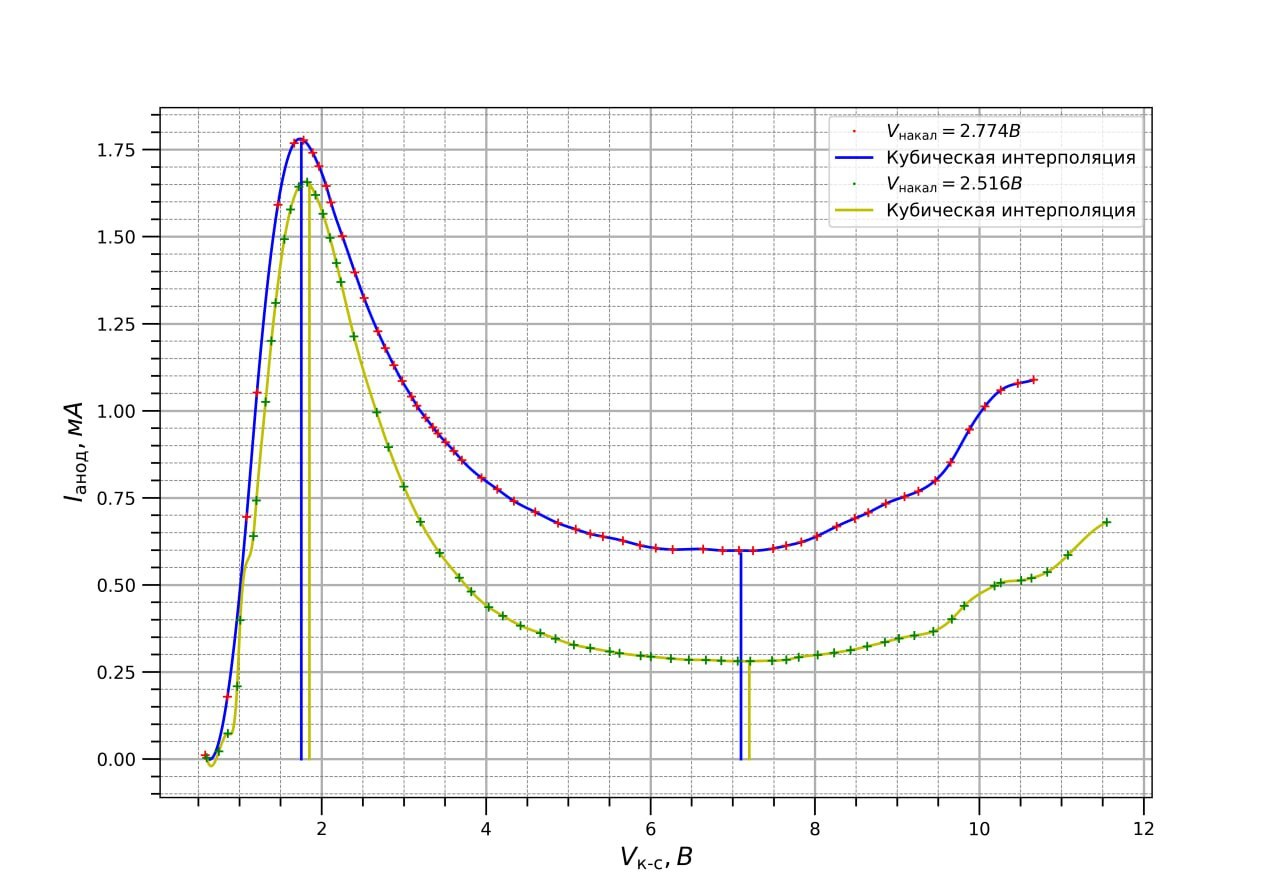
\includegraphics[width=1\linewidth]{1}
		\caption{График $ I_a = f(V_c) $ для двух значений напряжения накала}
	\end{figure}
	
	
	\item По графикам проведем те же измерения, что и в динамическом режиме. Полученные результаты занесем в таблицу 4.  
	\begin{longtable}{|c|c|c|c|}
		\hline
		& $\Delta_{max}$, В & $\Delta_{min}$, В & $\Delta_{\text{проб.}}$, В \\ \hline
		$V_1 = 2,774$ В & 1,779 & 7,248 & 10 \\ \hline 	
		$V_1 = 2,516$ В & 1,820 & 7,061 & 10 \\ \hline
		
		\caption{Значения напряжений при первом максимуме и минимуме анодного тока и напряжение пробоя.$\sigma_{\Delta_{max/min}} = 0,001$ В}
	\end{longtable}
	
	\begin{longtable}{|c|c|c|c|c|}
		\hline
		$l_1$, \AA & $l_2$, \AA & $l_3$, \AA & $U_0$, эВ & $l_{\text{табл.}}$, \AA\\ \hline
		2,99 $\pm0,04$& 2,95 $\pm0,04$& 2,92 $\pm0,07$& 2,43$\pm0,05$ & 1 \\ \hline
		\caption{Полученные значения для размера электронной оболочки атома ксенона в статическом режиме. }
	\end{longtable}
	
	
	\item На основе формулы $w(V) = -\dfrac{1}{C}\ln \dfrac{I_\text{a}(V)}{I_0}$ найдем зависимость вероятности рассеяния электронов от энергии и построим соответствующий график. 
	
	
	\begin{figure}[H]
		\centering
		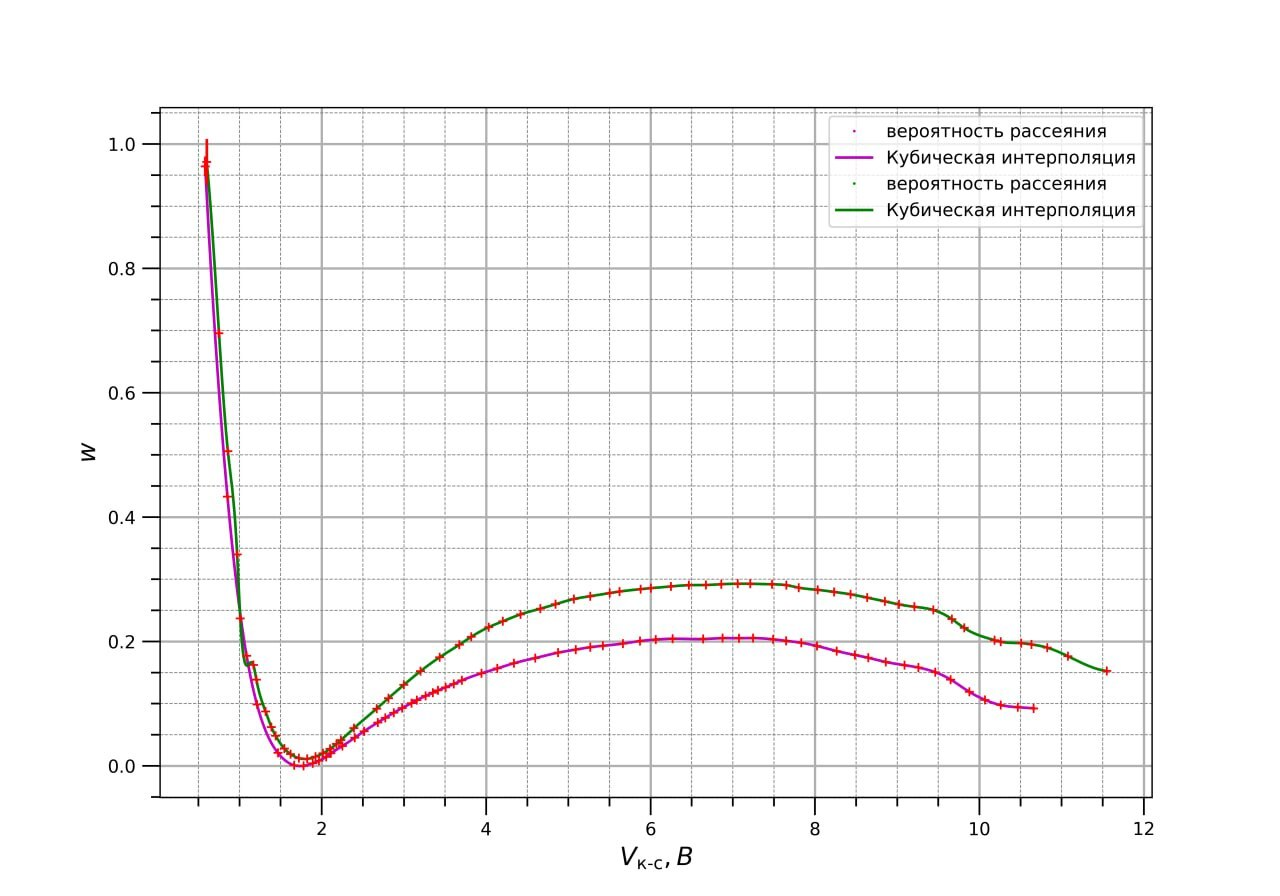
\includegraphics[width=1\linewidth]{2}
		\caption{График зависимости $w(V)$}
	\end{figure}
	
	\textbf{Обсуждение результатов и выводы: }\\
	
	В ходе данной работы мы исследовали энергетические зависимости рассеяния электронов атомами ксенона, определили энергии электронов при которых наблюдается просветление ксенона и оценили размер его внешней электронной оболочки.
	
	Измерения проводили динамическим и статическим методами. Полученные напряжения пробоя в динамическом режиме $ V_{\text{д}} = 12 \pm 0,5$ В и статическом $ V_{\text{с}} = 12,7 $ говорят о том, что используемый газ - ксенон ($ V_{\text{табл.}} = 12,1 $ В).
	
	Полученный по измерениям в динамическом режиме размер электронной оболочки $\overline{ l_{\text{д}}} \approx  3$ \AA, в статическом аналогично $\overline{ l_{\text{с}}} \approx  3$ \AA, что далеко от табличного значения для ксенона $l_{\text{табл.}} = 1$ \AA. Из чего можно сделать вывод, что использование одномерной потенциальной ямы для описания явления не подходит, а может использоваться только для оценки порядка величин.
	
	
	
	
	
	
	
	
	
	
	\end{enumerate}
	
	\end{document}